%\iffalse
\let\negmedspace\undefined
\let\negthickspace\undefined
\documentclass[journal,12pt,twocolumn]{IEEEtran}
\usepackage{cite}
\usepackage{amsmath,amssymb,amsfonts,amsthm}
\usepackage{algorithmic}
\usepackage{graphicx}
\usepackage{textcomp}
\usepackage{xcolor}
\usepackage{txfonts}
\usepackage{listings}
\usepackage{enumitem}
\usepackage{mathtools}
\usepackage{gensymb}
\usepackage[breaklinks=true]{hyperref}
\usepackage{tkz-euclide} % loads  TikZ and tkz-base
\usepackage{listings}



\newtheorem{theorem}{Theorem}[section]
\newtheorem{problem}{Problem}
\newtheorem{proposition}{Proposition}[section]
\newtheorem{lemma}{Lemma}[section]
\newtheorem{corollary}[theorem]{Corollary}
\newtheorem{example}{Example}[section]
\newtheorem{definition}[problem]{Definition}
%\newtheorem{thm}{Theorem}[section] 
%\newtheorem{defn}[thm]{Definition}
%\newtheorem{algorithm}{Algorithm}[section]
%\newtheorem{cor}{Corollary}
\newcommand{\BEQA}{\begin{eqnarray}}
\newcommand{\EEQA}{\end{eqnarray}}
\newcommand{\define}{\stackrel{\triangle}{=}}
\theoremstyle{remark}
\newtheorem{rem}{Remark}
%\bibliographystyle{ieeetr}
\begin{document}
%
\providecommand{\pr}[1]{\ensuremath{\Pr\left(#1\right)}}
\providecommand{\prt}[2]{\ensuremath{p_{#1}^{\left(#2\right)} }}        % own macro for this question
\providecommand{\qfunc}[1]{\ensuremath{Q\left(#1\right)}}
\providecommand{\sbrak}[1]{\ensuremath{{}\left[#1\right]}}
\providecommand{\lsbrak}[1]{\ensuremath{{}\left[#1\right.}}
\providecommand{\rsbrak}[1]{\ensuremath{{}\left.#1\right]}}
\providecommand{\brak}[1]{\ensuremath{\left(#1\right)}}
\providecommand{\lbrak}[1]{\ensuremath{\left(#1\right.}}
\providecommand{\rbrak}[1]{\ensuremath{\left.#1\right)}}
\providecommand{\cbrak}[1]{\ensuremath{\left\{#1\right\}}}
\providecommand{\lcbrak}[1]{\ensuremath{\left\{#1\right.}}
\providecommand{\rcbrak}[1]{\ensuremath{\left.#1\right\}}}
\newcommand{\sgn}{\mathop{\mathrm{sgn}}}
\providecommand{\abs}[1]{\left\vert#1\right\vert}
\providecommand{\res}[1]{\Res\displaylimits_{#1}} 
\providecommand{\norm}[1]{\left\lVert#1\right\rVert}
%\providecommand{\norm}[1]{\lVert#1\rVert}
\providecommand{\mtx}[1]{\mathbf{#1}}
\providecommand{\mean}[1]{E\left[ #1 \right]}
\providecommand{\cond}[2]{#1\middle|#2}
\providecommand{\fourier}{\overset{\mathcal{F}}{ \rightleftharpoons}}
\newenvironment{amatrix}[1]{%
  \left(\begin{array}{@{}*{#1}{c}|c@{}}
}{%
  \end{array}\right)
}
%\providecommand{\hilbert}{\overset{\mathcal{H}}{ \rightleftharpoons}}
%\providecommand{\system}{\overset{\mathcal{H}}{ \longleftrightarrow}}
	%\newcommand{\solution}[2]{\textbf{Solution:}{#1}}
\newcommand{\solution}{\noindent \textbf{Solution: }}
\newcommand{\cosec}{\,\text{cosec}\,}
\providecommand{\dec}[2]{\ensuremath{\overset{#1}{\underset{#2}{\gtrless}}}}
\newcommand{\myvec}[1]{\ensuremath{\begin{pmatrix}#1\end{pmatrix}}}
\newcommand{\mydet}[1]{\ensuremath{\begin{vmatrix}#1\end{vmatrix}}}
\newcommand{\myaugvec}[2]{\ensuremath{\begin{amatrix}{#1}#2\end{amatrix}}}
\providecommand{\rank}{\text{rank}}
\providecommand{\pr}[1]{\ensuremath{\Pr\left(#1\right)}}
\providecommand{\qfunc}[1]{\ensuremath{Q\left(#1\right)}}
	\newcommand*{\permcomb}[4][0mu]{{{}^{#3}\mkern#1#2_{#4}}}
\newcommand*{\perm}[1][-3mu]{\permcomb[#1]{P}}
\newcommand*{\comb}[1][-1mu]{\permcomb[#1]{C}}
\providecommand{\qfunc}[1]{\ensuremath{Q\left(#1\right)}}
\providecommand{\gauss}[2]{\mathcal{N}\ensuremath{\left(#1,#2\right)}}
\providecommand{\diff}[2]{\ensuremath{\frac{d{#1}}{d{#2}}}}
\providecommand{\myceil}[1]{\left \lceil #1 \right \rceil }
\newcommand\figref{Fig.~\ref}
\newcommand\tabref{Table~\ref}
\newcommand{\sinc}{\,\text{sinc}\,}
\newcommand{\rect}{\,\text{rect}\,}
%%
%	%\newcommand{\solution}[2]{\textbf{Solution:}{#1}}
%\newcommand{\solution}{\noindent \textbf{Solution: }}
%\newcommand{\cosec}{\,\text{cosec}\,}
%\numberwithin{equation}{section}
%\numberwithin{equation}{subsection}
%\numberwithin{problem}{section}
%\numberwithin{definition}{section}
%\makeatletter
%\@addtoreset{figure}{problem}
%\makeatother

%\let\StandardTheFigure\thefigure
\let\vec\mathbf

\bibliographystyle{IEEEtran}


\vspace{3cm}



\bigskip

\renewcommand{\thefigure}{\theenumi}
\renewcommand{\thetable}{\theenumi}
%\renewcommand{\theequation}{\theenumi}
Question : An urn contains 25 balls of which 10 balls bear a mark $X$ and the remaining 15 bear a mark $Y$. A ball is drawn at random from the urn, its mark is noted down and it is replaced. If 6 balls are drawn in this way, find the probability that\\
\begin{enumerate}[label=(\alph*)]
\item all will bear $X$ mark.\\
\item not more than 2 will bear $Y$ mark.\\
\item at least one ball will bear $Y$ mark.\\
\item the number of balls with X mark and $Y$ mark will be equal.\\
\end{enumerate}
\solution  \\
\begin{table}[!ht]
\centering
\begin{tabular}{|l|c|r|}
    \hline
    Parameter & Values & Description\\
    \hline
    $n$ & 6 & Number of draws\\
    \hline
    $p$ & 0.4 & Probability that ball bears $X$ mark \\
    \hline
    $q$ & 0.6 & Probability that ball bears $Y$ mark \\
    \hline
    $\mu=np$ & 2.4 & mean of the distribution \\
    \hline
    $\sigma=npq $ & 1.2 & variance of the distribution\\
    \hline
    $X$ &  & Number of cards bear mark $X$ \\
    \hline
    $Y$ &  & Number of cards bear mark $Y$ \\
    \hline
\end{tabular}
\caption{Definition of parameters}
\label{tab:gaussian/9/3/17}
\end{table}

\textbf{using Gaussian}
\begin{align}
Y \sim \gauss{\mu}{\sigma^2}
\end{align}
The CDF of $Y$:
\begin{align}
	F_Y(y) &= 1 - \pr{Y>y}\\
	&= 1 - \pr{\frac{Y-\mu}{\sigma}>\frac{y-\mu}{\sigma}}
\end{align}
But,
\begin{align}
	\frac{Y-\mu}{\sigma} &\sim \gauss{2.4}{1.44}\\
\end{align}
the Q-function is defined as:
\begin{align}
\qfunc{x} &= \pr{Y > x} \, \forall x \in Y \sim \mathcal{N}(2.4,1.44) 
\end{align}
therefore the cdf will be:
\begin{align}
F_Y\brak{y} &= 
\begin{cases}
           1-\qfunc{ \frac{y-\mu}{\sigma}}, &  y > \mu \\
           \qfunc{ \frac{\mu-y}{\sigma}} , &  y < \mu
\end{cases} 
\end{align}
\begin{enumerate}[label=(\alph*)]
\item all will bear $X$ mark.\\
\textbf{using Gaussian} \\
considering 0.5 as the correction term,\\
\begin{align}
\pr{X > 5.5} &= 1-F_X\brak{5.5} \\
             &=Q\brak{\frac{5.5-\mu}{\sigma}} \quad \\
             &= Q\brak{\frac{3.1}{1.2}} \\
             &= Q\brak{2.583} \\
             &= 0.00489
\end{align}
\item not more than 2 will bear $Y$ mark.\\  
\textbf{using Gaussian} \\
considering 0.5 as the correction term,\\
\begin{align}
\pr{Y < 2.5} &= 1-Q\brak{\frac{2.5-\mu}{\sigma}} \quad \\
             &= 1-Q\brak{\frac{-1.1}{1.2}} \\
             &= 1-Q\brak{-0.9166} \\
             &= Q\brak{0.9166} 
             &= 0.1796
\end{align}
\item at least one ball will bear $Y$ mark.\\
\textbf{using Gaussian} \\
considering 0.5 as the correction term,\\
\begin{align}
\pr{Y < 0.5} &= 1-Q\brak{\frac{0.5-\mu}{\sigma}} \quad \\
             &= 1-Q\brak{\frac{-1.1}{1.2}} \\
             &= 1-Q\brak{-2.588} \\
             &= 1-0.0048\\
             &= 0.9952
\end{align}
\item the number of balls with X mark and $Y$ mark will be equal.\\
\textbf{using Gaussian} \\
considering 0.5 as the correction term,\\
the gaussian distribution function is defined as:
\begin{align}
p_Y\brak{x} &= \frac{1}{\sqrt{2\pi{\sigma}^2}} e^{-\frac{\brak{x-\mu}^2}{2{\sigma}^2}}
\end{align}
the probability of the person winning the prize exactly once is given by:
\begin{align}
p_X\brak{3} &= \frac{1}{\sqrt{2\pi{\sigma}^2}} e^{-\frac{\brak{3-\mu}^2}{2{\sigma}^2}} \\
            &=\frac{ 0.882}{\sqrt{2\pi{\sigma}^2}}\\
            &=0.2933\\
 p_Y\brak{3} &= \frac{1}{\sqrt{2\pi{\sigma}^2}} e^{-\frac{\brak{3-\mu}^2}{2{\sigma}^2}} \\
            &= 0.2933\\
\pr{X=3 + Y=3}&=p_X\brak{3}p_Y\brak{3}\\
&=0.086
\end{align}
\end{enumerate}
\textbf{Gaussian vs Binomial Table}
\begin{table}[!ht]
\centering
\begin{tabular}{|l|c|r|}
    \hline
    Question & Gaussian & Binomial\\
    \hline
    all will bear $X$ mark & 0.00489 &0.00409\\
    \hline
   not more than 2 will bear $Y$ mark & 0.1796 & 0.1792 \\
    \hline
     at least one ball will bear $Y$ mark &  0.9952& 0.9959 \\
    \hline
    the number of balls with X mark and $Y$ mark will be equal& 2.4 & 0.2764\\
    \hline
\end{tabular}
\caption{Definition of parameters}
\label{tab:gaussian/9/3/17}
\end{table}

\textbf{Gaussian vs Binomial graph}
\begin{figure}[!ht]
\centering
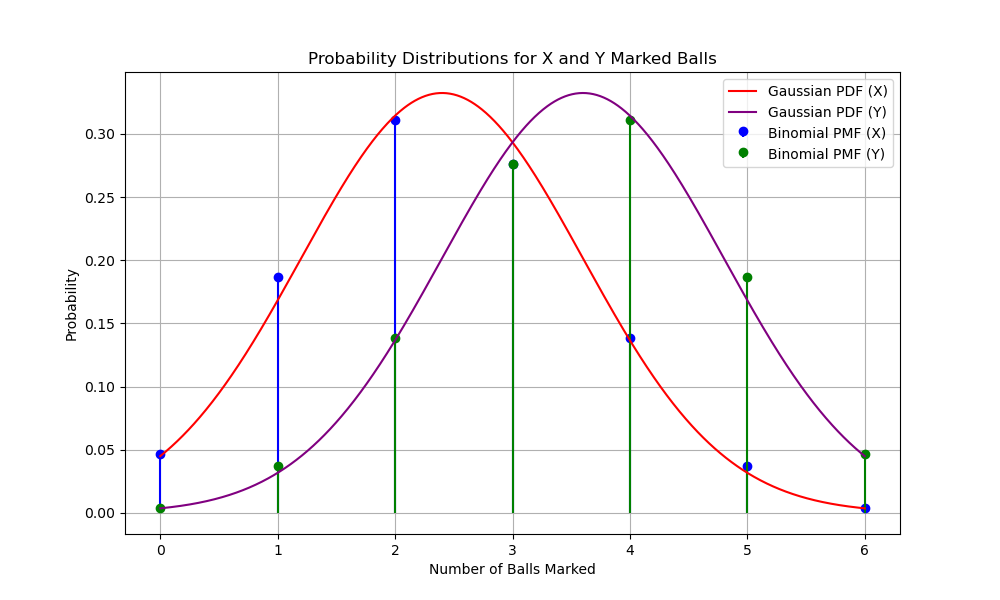
\includegraphics[width=\columnwidth]{/home/sravanthi/17/figs/Fig1.png}
\caption{pmf of binomial and pdf of Gaussian of X and Y marked balls}
\end{figure}
\end{document}
